\documentclass[10pt,twocolumn,letterpaper]{article}

\usepackage{cvpr}
\usepackage{times}
\usepackage{epsfig}
\usepackage{graphicx}
\usepackage{amsmath}
\usepackage{amssymb}
\usepackage{bm}

% Include other packages here, before hyperref.

% If you comment hyperref and then uncomment it, you should delete
% egpaper.aux before re-running latex.  (Or just hit 'q' on the first latex
% run, let it finish, and you should be clear).
%\usepackage[pagebackref=true,breaklinks=true,letterpaper=true,colorlinks,bookmarks=false]{hyperref}

\cvprfinalcopy % *** Uncomment this line for the final submission

\def\cvprPaperID{****} % *** Enter the CVPR Paper ID here
\def\httilde{\mbox{\tt\raisebox{-.5ex}{\symbol{126}}}}

% Pages are numbered in submission mode, and unnumbered in camera-ready
\ifcvprfinal\pagestyle{empty}\fi
\begin{document}

%%%%%%%%% TITLE
\title{W4735 Visual Interfaces to Computers\\Final Project Report: Real-time Gesture-based Game Control}
\author{Jie Huang and Shao-Chuan Wang\\
Department of Computer Science\\
Columbia University\\
{\tt\small \{jh3105, sw2644\}@columbia.edu}
% For a paper whose authors are all at the same institution,
% omit the following lines up until the closing ``}''.
% Additional authors and addresses can be added with ``\and'',
% just like the second author.
% To save space, use either the email address or home page, not both
}

\maketitle
\thispagestyle{empty}

%%%%%%%%% ABSTRACT
\begin{abstract}
In this report, we are going to introduce a system that exploits two bare hands image 
as visual input to control a real-time game. To find the user's hands in the captured colored image, 
we perform skin segmentation using hue-saturation 
thresholding on HSV color space. Since faces are also in skin color, we 
use face detection to prune the faces. 
We proposed an algorithm to find the fingertips as well as 
a control algorithm by analyzing the position and the orientation of a 
line between two fingertips; the position and the orientation of the line 
have a mapping to the controlled object on the screen. 
The development tools we used are python wrapper 
of OpenCV 2.1 library, and pygame for game development. Our codes 
can be downloaded from \verb"http://code.google.com/p/breakout/"
\end{abstract}

%%%%%%%%% BODY TEXT

\section{Introduction}
\label{sec:intro}

Visual interfaces in the applications of human-computer interface 
have been progressed tremendously in recent years. In particular, an outside-out 
visual system \cite{outout} which does not require players to wear 
any extra devices provides flexibilities in gaming applications, if 
the motion of the body can be accurately captured.
As we can see from the recent example, Microsoft Kinect, is the 
first vision-based commercial game platform, and it does 
create a lot of new paradigms for playing video games with human bodies. 

However, the idea of using gesture or human body as game
controllers appeared in 1990s. For example, 
Freeman et al. \cite{cvicg, cvfcg} implemented a computer vision based 
computer game system, based on image moments and orientation histograms, and 
use the chips to provide real-time interactive responses to the players. 

More recently, H\"{a}m\"{a}l\"{a}inen \cite{childgame} designed a perceptual user interface for
controlling a flying cartoon-animated dragon in a
physically and vocally interactive computer game for 4 to 9 years old children.
Lu et al. \cite{racecar} proposed a vision-based 3D racing car game controlling
method by analyzing the distance of two fists positions of the player
from the camera to control the direction of the racing car. Similarly, 
Schlattmann \cite{3dgames} et al. demonstrated three 3D real-time games via bare-handed 
interactions. All studies show higher usability via vision-based gesture controls 
in their usability tests.

Our work is motivated by Lu \cite{racecar} and 
Schlattmann \cite{3dgames}. We found that using bare-hands is particularly 
adaptable to the game control, especially for some category of games such as 
car driving. 

In this proposal, we propose to build a gesture-based game controller, which 
requires the modern computer vision technology. For a detailed review on visual 
interface of hand gestures and human motion capture, please see 
the review articles \cite{pamireview, cviureview}.

\section{Design decisions}
\subsection{Hardware}
\begin{table}[b!]
\begin{tabular}{c|ccc}
&High-end\\
&Camera&Web Camera&Kinect \\
\hline
Frame rates & fast & adequate & adequate \\
Resolution & HD 1080 & VGA & VGA \\
Availability & medium & high & low \\
Skin detection & not very easy & not very easy & very easy \\
Noises & low & high & medium \\
Cost & high & low & high 
\end{tabular}
\caption{The comparison between different capturing devices.}
\label{tab:hw}
\end{table}
Table~\ref{tab:hw} compares different hardware devices.
Our team considered to use Kinect to implement the system; however, 
we chose to use normal laptop web camera due to its availability as well as its 
low cost. 
Our webcams have frame rates ranging from 15fps to 30fps, which is adequate for real-time 
game control. Also, we need a colored camera in order to detect the skin color.


Since we chose low-end cameras as our capturing devices, we cannot design too 
complicated gesture grammar with small or fast movement. Fortunately, this 
constraint will not be a big problem for game control. We do not need complex 
commands in the game. As we will see in the later sections, we chose to find the 
blobs or convex hulls of user's hands, which does not require high-end cameras. 

\subsection{Software}
We used python as our developing programming language due to 
its dynamic and high-level properties. As introduced in the end 
of Section \ref{sec:intro}, we need modern computer vision 
techniques to \emph{recognize} the gesture commands. 
Python has OpenCV wrapper, we can try many existing computer vision 
algorithms without too much efforts. In addition, python 
is an interpreter and hence we can tune 
the parameters quickly without recompiling the whole system. 
Python has a game development package called pygame, which 
has event handling, sound handling, and screen drawing for producing 
games. To fulfill the needs to gesture-controlled game development, 
we find python has good library supports and is easy for rapid development.

As a brief summary, we chose python as our developing programming 
language due to the following reasons:
\begin{itemize}
	\item Python is cross-platform. We are developing on Mac OS and Windows simultaneously.
	\item Python is dynamic and high-level. Good for rapid development.
	\item Python is an interpreter. We don't need to recompile the codes as we are trying some parameters.
	\item Python has abundant library support such as OpenCV and pygame. 
\end{itemize}

In this project, we are focusing on the visual interface 
design. Hence, we do not intend to build a game from the scratch. 
Instead, we chose to modify an exisiting game which is open sourced. 
The original version of pybreakout can be downloaded at
\verb"http://code.google.com/p/pybreakout/"

\subsection{Game: breakout}
We chose an ancient Nintendo game \emph{Breakout} and modified 
the way we control the paddle. Traditionally, the paddle can 
move only horizontally along a predetermined line at a constant speed.
In our design, we chose to enable the paddle to move upward and rotate.
We guess the reason why the traditional design did not incorporate 
rotation is that 
it is not intuitive to rotate the paddle with gamestick.
\begin{figure}[h]
\centering
\begin{tabular}{cc}
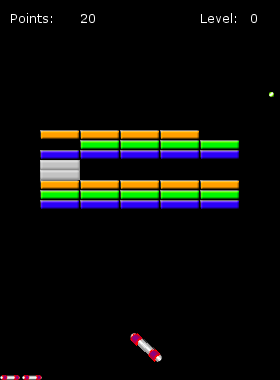
\includegraphics[height=3.5cm]{game0060.png} &
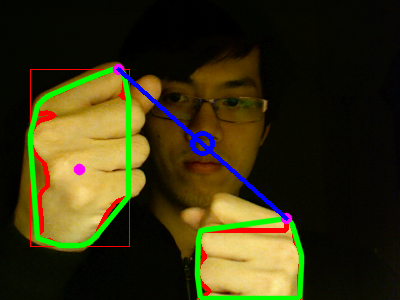
\includegraphics[height=3.5cm]{gesture0060.png} \\
(a) Game play screen &
(b) Control screen
\end{tabular}
\caption{A screenshot of playing \emph{breakout}}
\label{fig:gamescreen}
\end{figure}

However, if we control the orientation and position of the paddle 
using the gesture shown in Figure~\ref{fig:gamescreen} (b), 
we can control the paddle according to our gesture commands.

Figure~\ref{fig:gamescreen} (b) shows our design of control. 
We used tips of two bare hands as references, and the orientation and 
the position of the paddle is controlled by the blue line in 
Figure~\ref{fig:gamescreen} (b). We can see that in Figure~\ref{fig:gamescreen} 
(a) and (b), the paddle and the blue line has the same orientation.

We can also easily extend this controlling interface to other 
games such as car driving games due to the fact that in most 
car driving games, we only need to control the wheel by 
orientation. It would be also very intuitive to control 
the virtual car using two bare hands, as shown in Figure~\ref{fig:cargame}.
\begin{figure}[h]
\centering
\begin{tabular}{cc}
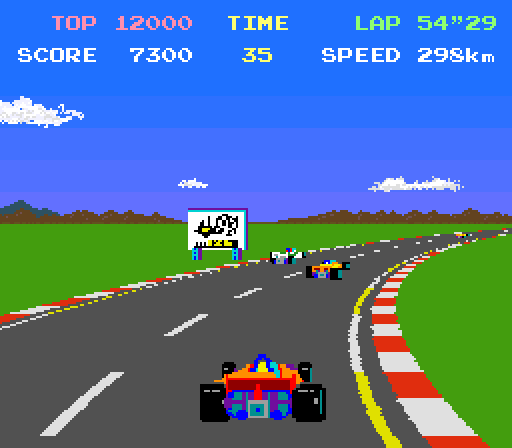
\includegraphics[height=3cm]{cargame.png} &
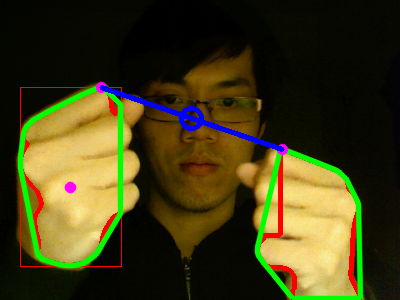
\includegraphics[height=3cm]{gesture0047.png} \\
(a) A car game screen &
(b) Control screen
\end{tabular}
\caption{A concept screenshot of playing a car game.}
\label{fig:cargame}
\end{figure}

\subsection{Machine-human interface: Bare hands}
\label{sec:whybarehands}
We chose to use bare hands as our machine-human interface 
to control the game play due to the following reasons:

\begin{itemize}
	\item It is too cubersome to wear any extra devices/markers.
	\item We can extend our work of assignment one.
	\item It is more intuitive to use your own hands to control the game.
	\item You do not have to find and setup the devices before you play.
\end{itemize}

However, it also have disadvantages, and to name a few,
\begin{itemize}
	\item Skin segmentation is not robust.
	\item Images from the webcamera is mostly noisy.
	\item The environment becomes rather restricted. We cannot play in all kinds of environments.
\end{itemize}
To compensate the environment issues, we designed an user-interface 
to adjust the parameters to adapt to different lighting environment as shown in Figure~\ref{fig:adjusting}. 

\begin{figure}[h]
\centering
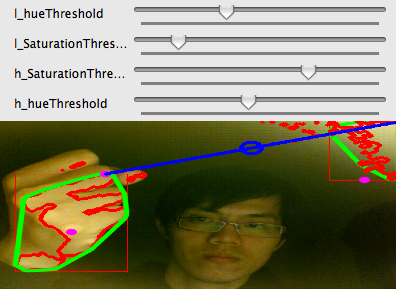
\includegraphics[width=7cm]{adjustui.png}
\caption{A screenshot on the user interface to adjust parameters. We provide 
sliders to adjust system parameters.}
\label{fig:adjusting}
\end{figure}

More details on skin detection will be explored in Section \ref{sec:gesture}.

\subsection{System overview}
(block diagrams) and how visual interface invoke the movement.

\section{Gesture controller}
\label{sec:gesture}
We have several submodules to implement the gesture controller.

\subsection{Skin detection}
\label{sec:skin}
\paragraph{Step 1: Gaussian blur}
Blurring makes the input image smoother such that we can get more complete contours. 
We started with a median filter using a $17 \times 17$ aperture based on our homework 1 experience. 
We then realized $17 \times 17$ aperture is too slow for the real-time controller. Therefore, we 
changed to a Gaussian filter with $5 \times 5$ Gaussian kernel. And we ran the filter for 4 times 
to achieve the similar result as a $17 \times 17$ median filter. It turns out even running 4 times 
is much faster than running a median filter with large aperture.

Sample OpenCV code:
\begin{verbatim}
cv.Smooth(bgrimg, img_temp, 
       cv.CV_GAUSSIAN, 5, 5)
\end{verbatim}

\begin{figure}[h]
\centering
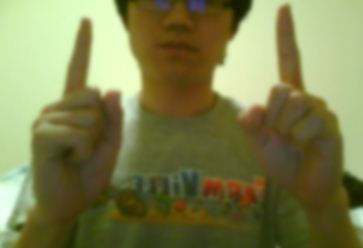
\includegraphics[width=7cm]{gaussian.png}
\caption{An example of gaussian blurred image.}
\label{fig:gaussin}
\end{figure}

\paragraph{Step 2: Color filtering in HSV color space} In this step,  
we convert the blurred RGB image into HSV color space. In homework 1 we used 
hue(H) and intensity(V) to identify the skin color, with the help of external illumination 
to intensify the V value of hand skin. However, in this project, we want to reduce the 
dependencies on the environment colors and lights, so that our game can be played in different 
settings.

We found that using saturation (S) channel is more suitable for this purpose 
than V channel since saturation is more stable in different settings than intensity. 
Though it still has much dependency on the environment, we do not need the help of 
the external illumination. As described in later sections, we will use other 
additional measures to improve the detection accuracy. 

Sample OpenCV code:
\begin{verbatim}
# Convert to HSV color space
cv.CvtColor(bgrimg, hsvimg, cv.CV_RGB2HSV)
# Find regions with skin colors
cv.InRangeS(hsvimg, low, high, skin_mask)
\end{verbatim}

\begin{figure}[h]
\centering
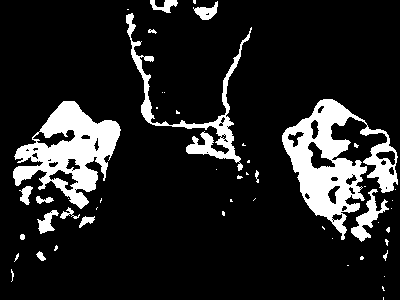
\includegraphics[width=7cm]{hsv.png}
\caption{Skin detection in HSV color space.}
\label{fig:hsv}
\end{figure}

\subsection{Motion detection}
As described above, color-based skin detection has dependency on the environment. 
We need additional instruments to help with more accurate gesture detection. As our 
game controlling events are issued by the movement of hands, it is natural to use motion 
detection to help with the gesture detection. The process is as follows:
We keep a buffer of 10 history frames most recently captured by the camera, 
and for every new incoming frame, we calculate the difference with the last frame 
to get the difference image. We then apply threshold the difference image to discard 
the small values, which are likely introduced by noises or movement within the 
silhouettes. The resulting image we got represents the moving silhouettes over the 
last two frames.

Sample OpenCV code:
\begin{verbatim}
cv.AbsDiff(self.buf[-1], 
           self.buf[-2], self.silh)
cv.Threshold(self.silh, self.silh, 
       diff_threshold, 1, cv.CV_THRESH_BINARY)
\end{verbatim}

We then use the obtained moving silhouettes to update the motion history,
\begin{verbatim}
cv.UpdateMotionHistory(self.silh, 
      self.mhi, self.timestamp, 
      self.MHI_DURATION)
\end{verbatim}

The following formula describes how what 'UpdateMotionHistory' does:

\begin{equation}
mhi(x, y) = \begin{cases} timestamp, & \mbox{if silhouette(x, y)} \neq 0 \\ 
                          0, & \mbox{if silhouette(x, y)} = 0 \\
			  & \mbox{ and } \\
			  & mhi < (timestamp - duration) \\
			  mhi(x, y),  & \mbox{otherwise}.
			  \end{cases}
\end{equation}
The result matrix contains the motion information represented by timestamps. 
Only the points which are covered by moving silhouettes in recent frames 
have non-zero values. We can use the following function to scale the timestamps 
in the matrix to displayable range (0, 255).

\begin{verbatim}
param = (self.MHI_DURATION - \
      self.timestamp)*255 \
      /self.MHI_DURATION
cv.CvtScale(self.mhi, self.mask, 
        255/self.MHI_DURATION,
        param)
\end{verbatim}

The resulting image is the motion image, shown in Figure~\ref{fig:motion}
\begin{figure}[h]
\centering
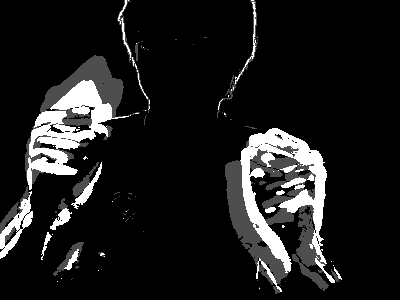
\includegraphics[width=7cm]{motion.png}
\caption{Motion history image.}
\label{fig:motion}
\end{figure}

Once we get the motion image, we segment it to get the major motions 
and discard the minor ones. The largest motions are supposed to be the moving hands.
\begin{verbatim}
seq = cv.SegmentMotion(self.mhi, 
        self.segmask, self.storage, 
        self.timestamp,
        self.MAX_TIME_DELTA) 
\end{verbatim}
Once we get the sequence of the motion segments, we can compare 
their areas to find the largest motions. The final mask 
contains simple rectangles specifying the regions with the most 
significant motions (as illustrated in the following image). The 
mask can be applied to the original blurred image, so that all 
the later calculations can focus on the white areas.
\begin{figure}[h]
\centering
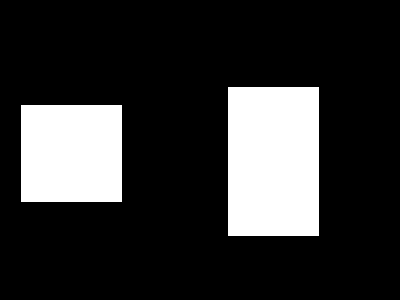
\includegraphics[width=7cm]{block.png}
\caption{An example of motion mask.}
\label{fig:motionmask}
\end{figure}

Our system implemented motion detection, and 
the experiment shows that, with motion detection enabled, 
the system is more reliable in noisy environment with color 
disturbances. However, considering the performance penalty, we 
disable motion detection feature by default.

\subsection{Face pruning}
\label{sec:face}
We described how we use hue and saturation thresholding to detect skin
 color and therefore find the hands; however, faces are also in skin color. 
 The user's face becomes a noise as we interpret the found skin mask as 
 two hands. We may assume that faces are bigger than hands and use 
 the area to filter out the faces. However, this criterion is not robust. 

 Hence, we chose to use OpenCV builtin face detection to find the faces 
 and wipe it out on the skin mask.

Sample OpenCV code:
 \begin{verbatim}
faces = cv.HaarDetectObjects(
           cv.GetMat(grayscale), 
	   cascade, 
	   storage, 
	   1.2, 2, 0, 
	   (100, 100))
 \end{verbatim}

Figure~\ref{fig:facedetect} shows a demo on face detection of OpenCV. 
We can see that it does find the user's face and did not 
falsely recognize the hands as faces.

 \begin{figure}[h]
 \centering
 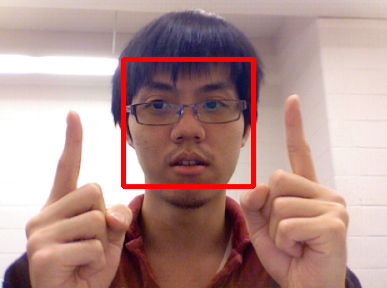
\includegraphics[width=7cm]{facedetection.png}
 \caption{The face detection of OpenCV unit testing. }
 \label{fig:facedetect}
 \end{figure}

With the rectangle of faces, we can prune the faces so that 
the later calculation will not need to consider them.


\subsection{Fingertips detection}
In this step, we aim to find the two fingertips (or fist tip, 
one from each hand). Input to this step is the binary image 
filtered by skin detection, face pruning and optional the motion mask.

We first find the contours in the image and from them pick the 
largest two contours (largest in the sense of area). They should 
be the contours of player’s hands. 

\begin{verbatim}
contours = cv.FindContours(im,.
              storage,
              cv.CV_RETR_EXTERNAL,
              cv.CV_CHAIN_APPROX_SIMPLE)
\end{verbatim}

We then simply pick the top point of each contour, and that 
should be the finger point we want to find.

The best point of using the fingertips is, it can tolerate 
considerable disturbances of skin detection and works quite 
well for only partially detected hands, as shown in Figure~\ref{fig:fingertip}

\begin{figure}[h]
\centering
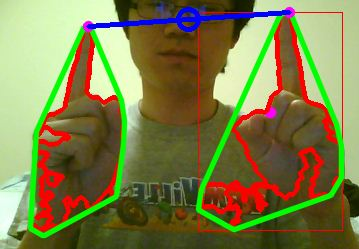
\includegraphics[width=7cm]{fingertip.png}
\caption{Color disturbance.}
\label{fig:fingertip}
\end{figure}

\begin{figure}[h]
\centering
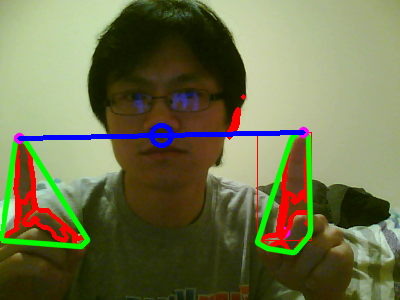
\includegraphics[width=7cm]{partialhand.png}
\caption{Partially detected hands}
\label{fig:partial hand}
\end{figure}

\subsection{Controller algorithms}
Now that we have the two fingertips, we can generate game 
controlling signals according to the movements of the two points. 
The movement (right/left, up/down) is controlled by the 
displacement of the center point of the two fingertips, and 
the rotation is controlled by the rotation of the line connecting 
the two fingertips. 

There are several issues for us to solve in order to achieve stable and smooth controlling experience.

\paragraph{Vibrations and very fast movements} 
Since there are always some little motions of hands even if the players try very hard 
to hold their hands still. Besides, the noise of the camera and the changing environment 
can also create small motions of the detected fingertips. On the other hand, too fast 
hand movements over two frames are usually not caused by players' hand movements. 
For example, it can be due to a sporadic wrong detection of one of the finger point. 

Considering of this, we set the minimum and maximum limit for the hand movement 
speed (currently minimum = 5 and maximum = 50 pixels/frame). Movements with speed 
out of this range will be discarded.

\paragraph{Abnormal movements}
As mentioned, sporadic wrong detection of the fingertips may happen from time 
to time. Even after we set the upper and lower limit of the moving speed, the 
abnormal detection may span more than two frames. Then, though the first frame with 
the abnormal detection will be discarded because it is beyond the legal movement 
speed range, the second will not because its speed is calculated based on its 
previous frame which has the same abnormal detection.

\begin{figure}[h]
\centering
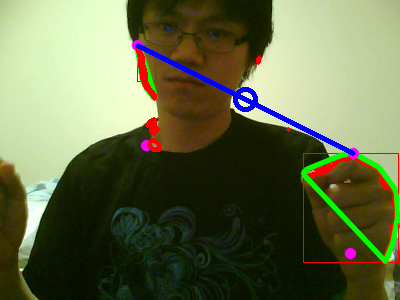
\includegraphics[width=7cm]{abnormal.png}
\caption{A sample of sporadic abnormal movement.}
\label{fig:abnormal}
\end{figure}

To solve this problem, we keep a list of 5 most recent history positions 
(of the center of the two fingertips), and another buffer of the same size 
to cache the abnormal center positions.  For each new frame, if the displacement 
is within the legal range, we go ahead to trigger the move/rotation events, 
and clear the abnormal buffer. Otherwise, if the displacement is larger than 
the upper limit, we place it in the abnormal buffer. Then we scan the abnormal 
buffer, if all the 5 points in it are one by one adjacent, we accept the abnormal 
position as the new position and replace the history buffer with the abnormal 
buffer. And as well, issue the movement events accordingly. (This usually 
indicates that the player moved her/his hands very quickly to a different region.)

By using this two buffer strategy, most of the sporadic wrong detections are filtered, and the game controlling is largely smoothed. Following is the code of the core algorithm:

{\tiny{
\begin{verbatim}
# The method is generate game controlling 
# signals, the parameter polar is the in 
# the form of ((x,y), theta), where (x,y) 
# is the center of the fingertips, and 
# theta of the radian of the fingertips line
def update_game(self, polar):
      last = self.history[-1]
      degree_change = abs(polar[1] - last[1]).
      p1 = last[0]
      p2 = polar[0]
      # the position change from the last
      pos_change = util.get_point_distance(p1, p2)

      # if the displacement is beyond the legal range
      if pos_change > self.max_pos_change or \
              degree_change > self.max_degree_change: 
              # add to abnormal buffer
              self.buf.append(polar)
              if len(self.buf) > self.history_size:
                  self.buf.pop(0) 
              if self.__check_buffer_stable():
                  print "buf is determined to be stabe, replace history with buf"
                  self.history = self.buf
                  self.buf = []
              else:
                  print "buf is not stable, this move is abandoned."
                  return
      else:
          # add to history buffer
          self.history.append(polar)
          self.history.pop(0)
          self.buf = []  # clear abnormal buffer
      # code for issue game controlling events ignored
      # …
      # …

# Check whether all the points in the buffer are adjacent to the next
def __check_buffer_stable(self):
     stable = True
     # return immediately if the buffer is not full
     if len(self.buf) < self.history_size: return False 
     for i in range(self.history_size - 1):
         p1 = self.buf[i][0]
         p2 = self.buf[i+1][0]
         d1 = self.buf[i][1]
         d2 = self.buf[i+1][1]
         # center distance = movement speed
         delta_p = util.get_point_distance(p1, p2) 
         # angle distance = rotation speed
         delta_d = abs(d1 - d2)   
         if delta_p > self.max_pos_change or \
                 delta_d > self.max_degree_change:
             stable = False
     return stable
\end{verbatim}
}}

\section{Alternative designs of interface}
% rectangle in the center.
% not bare hands
\subsection{One-hand controller}
Our initial design is to control the game with one hand instead of two. 
The movement can follow the center of the hand, and the rotation can be 
controlled by the left and right rotation of the index finger (as shown in 
Figure~\ref{fig:singlehand}).

\begin{figure}[h]
\centering
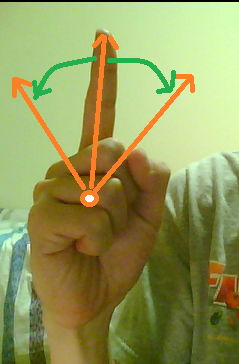
\includegraphics[height=6cm]{singlehand.png}
\caption{Single hand controller}
\label{fig:singlehand}
\end{figure}

There are several major problems of this design:
\begin{itemize}
	\item It is hard for the index finger to rotate for a large angle.
	\item Sometimes the player wants only to rotate without movement. 
	But with this design, players cannot keep the hand center still when rotating. 
\end{itemize}

\subsection{Motion-only controller}
We also considered using controller which bases on motion detection only. 
Though motion detection is good for finding the interesting area (thus good 
for creating a mask), the contours found by it change frequently frame by frame. 
Therefore, we cannot find a stable point basing on which the movement can be measured.

\subsection{Control panel controller}
One considerable design is to use a control panel with 8 predefined regions 
in the frame (up, down, left, right, up-left, up-right, down-left and down-right) 
as shown in 

\begin{figure}[h]
\centering
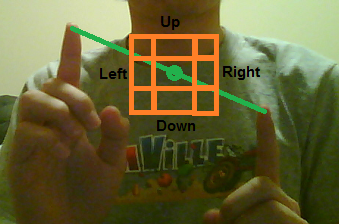
\includegraphics[width=7cm]{controlpanel.png}
\caption{Control panel controller.}
\label{fig:controlpanel}
\end{figure}

If the center of the fingertips is in the up region, the controller 
will keep sending move-up signals to the game, and similarly for the other 
regions. The rotation is still controlled by the angle of the fingertip line.
\paragraph{Advantages}
In this way, the movement could be very smooth and the unintended minor movements can easily be avoided.
\paragraph{Disadvantages}
Players need to pay much more attentions towards the control panel while playing the game. And it is hard to move quickly and accurately between different regions. (For example, from the upper-left region to the bottom-right region)

\subsection{Not bare hands}
Depending on the environment, the fingertip detection is not perfect in many settings. 
To improve the accuracy, we can use tools like finger cots as shown in the class. 
But in real life, no players would be happy to play the game with those additional tools. 
The decision of using bare hands in our design is discussed in Section \ref{sec:whybarehands}.

\section{Game perspectives}

\section{System optimization}
% resize
% cache (e.g. face training data)
% game tick vs control tick
A game control interface has to be real-time. In other words, 
the gesture decision has to be made in a very short period of time. 
We faced efficiency issues as we integrate the visual interface and 
the game. We found several ways to optimize the systems without 
sacrifacing the control accuracy.

\paragraph{Resize visual input.} The resolution of 
original visual input image is $640 \times 480$. 
We resize it to $400 \times 300$, and the speed boosted.
We do not need high-resoluted image because we detected 
blobs and contours which do not highly depend on image resolution. 
(the details of detecting the hands are depicted in Section 
\ref{sec:skin}.

\paragraph{Cache.} We do not calculat everything on the fly. 
If something can be done offline, we will precompute it and 
load it as the system starts. For example, in Section 
\ref{sec:face} we filtered out faces by face detection. 
The training face data are loaded only once at the beginning. 
In this way, we reduced the I/O overheads. We also did the 
similar cache for other resources.

\paragraph{Drop frames.} The computation of visual input 
and processing is heavier than the game; To smoothen the game 
play, we drop frames of visual input. We do not ask 
the visual interface to invoke the movement events. 
Hence, we sacrifaced the response time of the visual control 
without sacrifacing the frame rates of the game. In our 
current implementation, the ratio of the frame rates between 
visual control and game is $1/4$.

\section{System limitation}
% wide lens

\subsection{Noisy skin detection results}

\subsection{Control usability}

\section{Conclusion and future direction}
Our visual controlling interface can be applied to other games, 
such as car racing games. Our system have relatively stable control on 
orientation of two hands, and the orientational inforamtion can be 
used to control the direction of the racing car.

{\small
\bibliographystyle{ieee}
\bibliography{egbib}
}

\end{document}
